Processes like Powder Bed Fusion (PBF), similar to all industrial processes, possess parameters that ensure their proper functioning and control. When a process demonstrates the expected behavior, it's referred to as "in-control". On the other hand, when the process deviates from the desired behavior, the process's output becomes unpredictable, and it's referred as "out-of-control" (OOC). When a process is out of control, anomalies and defects can arise in the printed piece. In this section, we will delve into the most common defects in PBF processes in Section \ref{sec:defects}, and their causes. Lastly, we will focus on defects stemming from anomalies in the temperature profiles of the building bed in Section \ref{sec:hotspot}, which will aid in better comprehension of the subsequent sections. Sections of this chapter are mainly based on \citeauthor{grasso_-process_2017} (2017), \citeauthor{grasso_process_2017} (2017), \citeauthor{mostafaei_defects_2022} (2022) and \citeauthor{wu_additively_2023} (2023). Finally, In Section \ref{sec:comelotrovo} I will describe different approaches for defects detection, while in Section \ref{sec:sensoriniiniini} I will describe available sensors used in anomalies detection. 

% Categories of Defect in PBF Processes >>>
\section{Defects Categories and Causes in PBF Processes}
\label{sec:defects}
In this section, we will discuss the most common defects that can occur during a PBF printing process and their main causes.
\paragraph{Porosity.} Porosity is a really significant parameters for many metal AM applications, as it strongly on fatigue resistance and the attributes of crack propagation in the component \cite{edwards_electron_2013}. 
\begin{figure}
    \centering
    \subfloat[\label{fig:poris}]{
        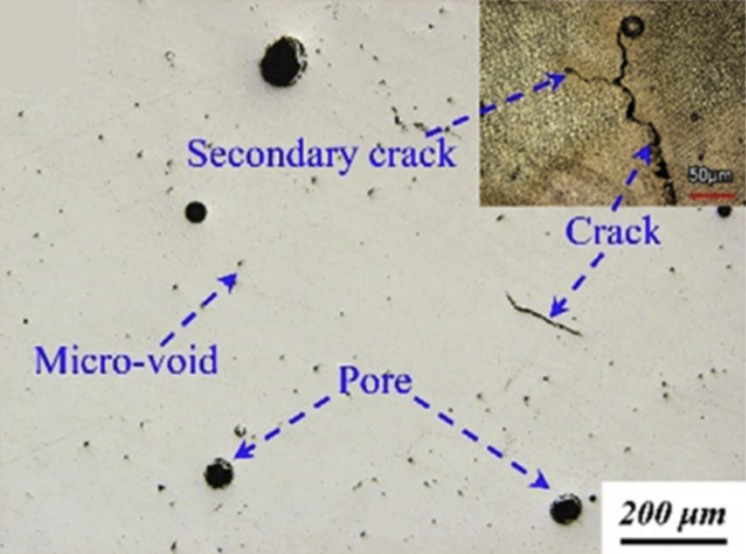
\includegraphics[scale=0.4]{Images/pori e crack.png}
    }
    \qquad
    \subfloat[\label{fig:acircular}]{
        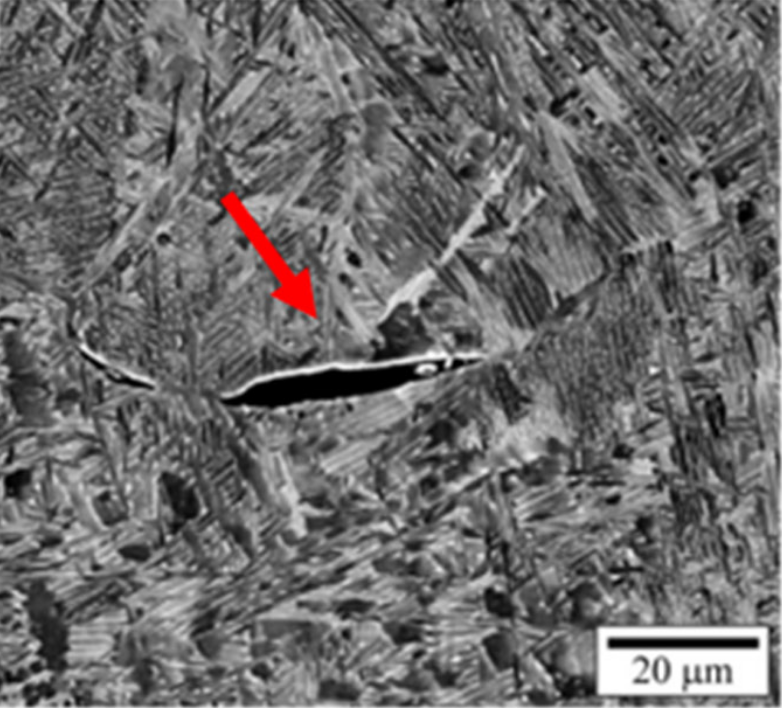
\includegraphics[scale=0.31]{Images/acircular.png}
    }
    \qquad
    \subfloat[\label{fig:delamination}]{
        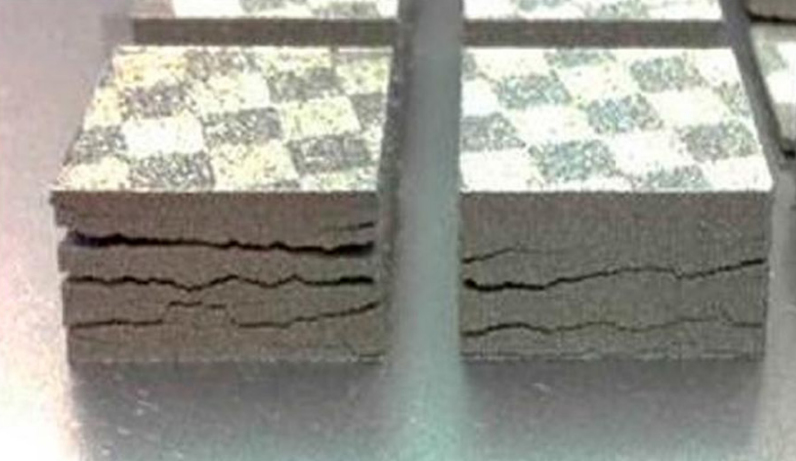
\includegraphics[scale=0.4]{Images/delamination.png}
    }
    \qquad
    \subfloat[\label{fig:balling}]{
        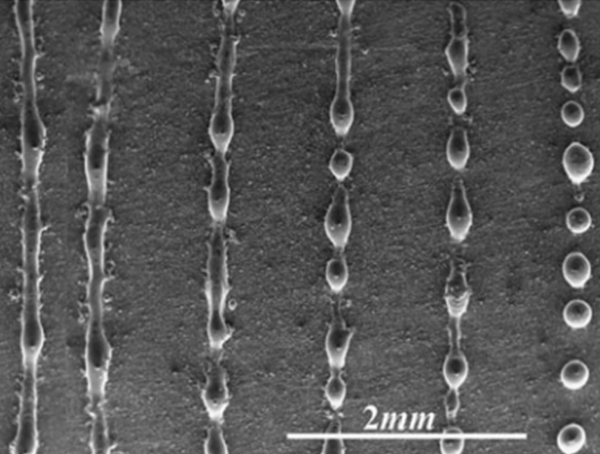
\includegraphics[scale=0.4]{Images/balling.png}
    }
    \caption[Defect examples in PBF.]{Pores, micro-void and cracks in a specimen of FeCrCoMnNi (a) \cite{mostafaei_defects_2022}, an acircular pores on a specimen of Ti–6Al–4V (b) \cite{tammas-williams_xct_2015}, an example of delamination in SLS (c) \cite{sames_metallurgy_2016} and the balling effect in stainless steal powder (d) \cite{li_balling_2012}.}
\end{figure} 
Porosity is characterized by empty spaces within the mass of the fused material. These voids can appear within a layer, between adjacent layers, or on the component's outer surface. Voids most frequently appear within the layer and can vary in size, form, and arrangement. The primary causes for these pores include incomplete fusion in the powder bed (lack of fusion or LOF), keyhole effects, and encapsulated gas. We can also differentiates between round and non-round pores. Some examples of round pores can be seen in Fig. \ref{fig:poris}. The elongated voids observed between layers are labeled as 'acicular pores' and they are recognized by their stretched form and larger size. For example, the acircular pore in Fig. \ref{fig:acircular} has a measure of \SI{20}{\micro\metre}. Pores can either be dispersed throughout the material or primarily situated between the inner patterned area and the outer boundary, known as under-skin pores. Pores can also appear on the exterior surface, where they are typically termed 'surface porosity'.
\paragraph{Residual stresses, cracking and delamination.} In material science, residual stresses are internal tensions that remains in the finished pieces also once the printing phase is complete. In PBF, this stresses can arise from two different causes: the thermal gradient mechanism and the cool-down phase of molten top layers \cite{mercelis_residual_2006}.Cracking phenomena occurs as a consequence of a stress relief when the tensile stress exceeds the ultimate tensile strength of the solid material. An example of cracking can be seen in \ref{fig:poris}. When the tension is suddenly released, a secondary crack can generate from the main crack. Delamination is a particular case of cracking, where cracks originate and propagate between adjacent layers (inter-layer cracking), when the residual stresses exceed the binding ability between the top layer and the previous one. Most of the times, delamination happens from the partial disconnection of the part from the baseplate \cite{sames_metallurgy_2016}, as in Fig. \ref{fig:delamination}.
\paragraph{Geometric defects and dimensional accuracy.} Dimensional anomalies in PBF can be categorized into (i) contraction and expansion effects, (ii) warping and curling, (iii) dross formation on bottom-facing surfaces, (iv) super-elevated edges, and (v) additional on-plane geometric distortions. Contraction is among the more common defects, though the contrasting effect (i.e., components that are consistently bigger than expected) might arise in certain scenarios. Warping predominantly stems from heat dispersion processes and thermal tensions. In a similar way, curling is a specific bending effect caused by inconsistent thermal growth and component shrinkage, generally tied to disparate contraction rates between the top and underside of overhanging segments. A combination of shrinking and warping effects results in curved outlines for bottom-facing surfaces intended to be flat. When confronted with bottom-facing facets, dross accumulation and flawed perimeters have been attributed to the absence or incorrect planning of support frameworks. RSuper-elevated edges represent another type of out-of-plane geometrical distortion, featured by elevated ridges of solidified material. These elevated edges not only compromise the final component's integrity but might also be the cause for defects propagation, since they can interfer with recoating blade syst. Other distortions affect critical features such as thin walls, overhang areas and acute corners. In correspondence of these features, the melt pool is largely surrounded by loose powder, which has a lower conductivity than the solid material. The diminished heat flux yields local over-heating phenomena that may deteriorate the geometric accuracy. This overheated area are called hot spot (HS) and will be discussed in Section \ref{sec:hotspot}.
\paragraph{Balling.} Melt ball formation, a.k.a. balling, occurs when the molten material solidifies into spheres instead of solid layers. This phenomenon is caused by surface tension, which prevents the molten material to wet the underlying layer. The result is a rough and bead-shaped surface that produces an irregular layer deposition, with detrimental effects on the density and quality of the final product. \citeauthor{li_balling_2012}(2012) pointed out three main problems when balling happens: increased surface roughness, large number of pores between the discontinuous metallic balls, and the spheres protruding may interfer with the recoating blade. The latter happens only in presence of a very severe balling. Fig. \ref{fig:balling} show the balling effect on a stainless steal powder.
\paragraph{Surface defects.}
\begin{figure}
    \centering
    \subfloat[\label{fig:lackofsupport}]{
        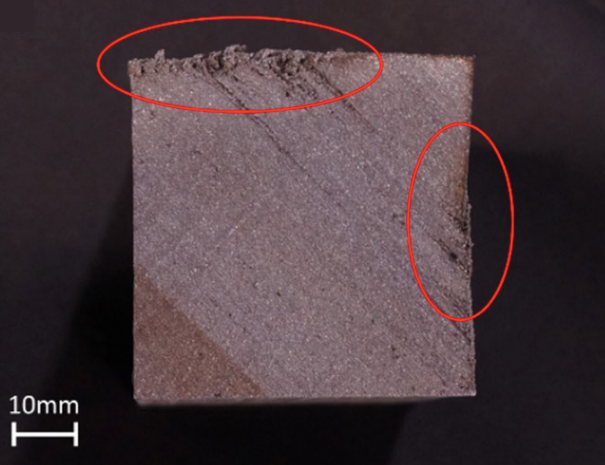
\includegraphics[scale=0.45]{Images/lackofsupport.png}
    }
    \qquad
    \subfloat[\label{fig:oxide}]{
        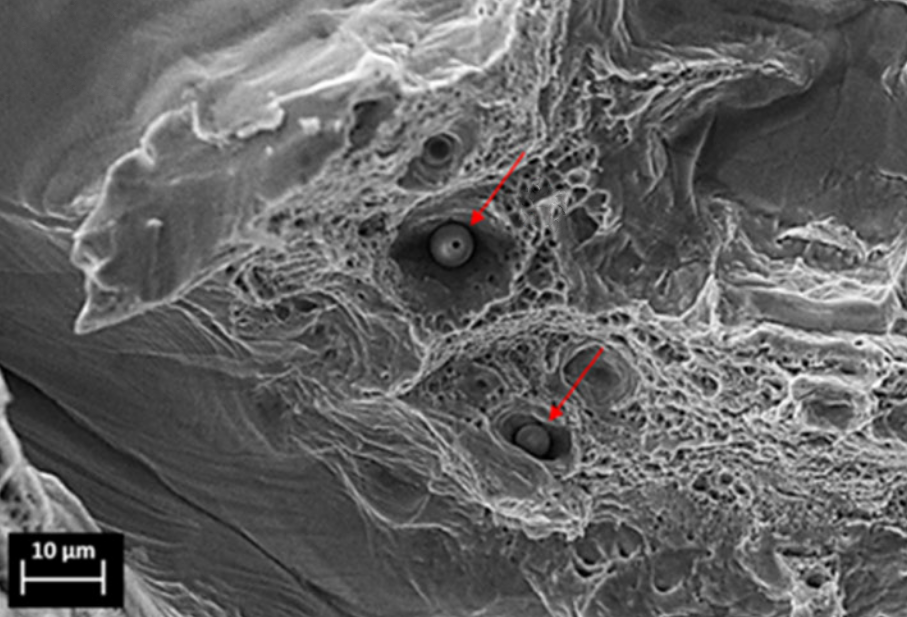
\includegraphics[scale=0.34]{Images/oxide.png}
    }
    \qquad
    \subfloat[\label{fig:surface}]{
        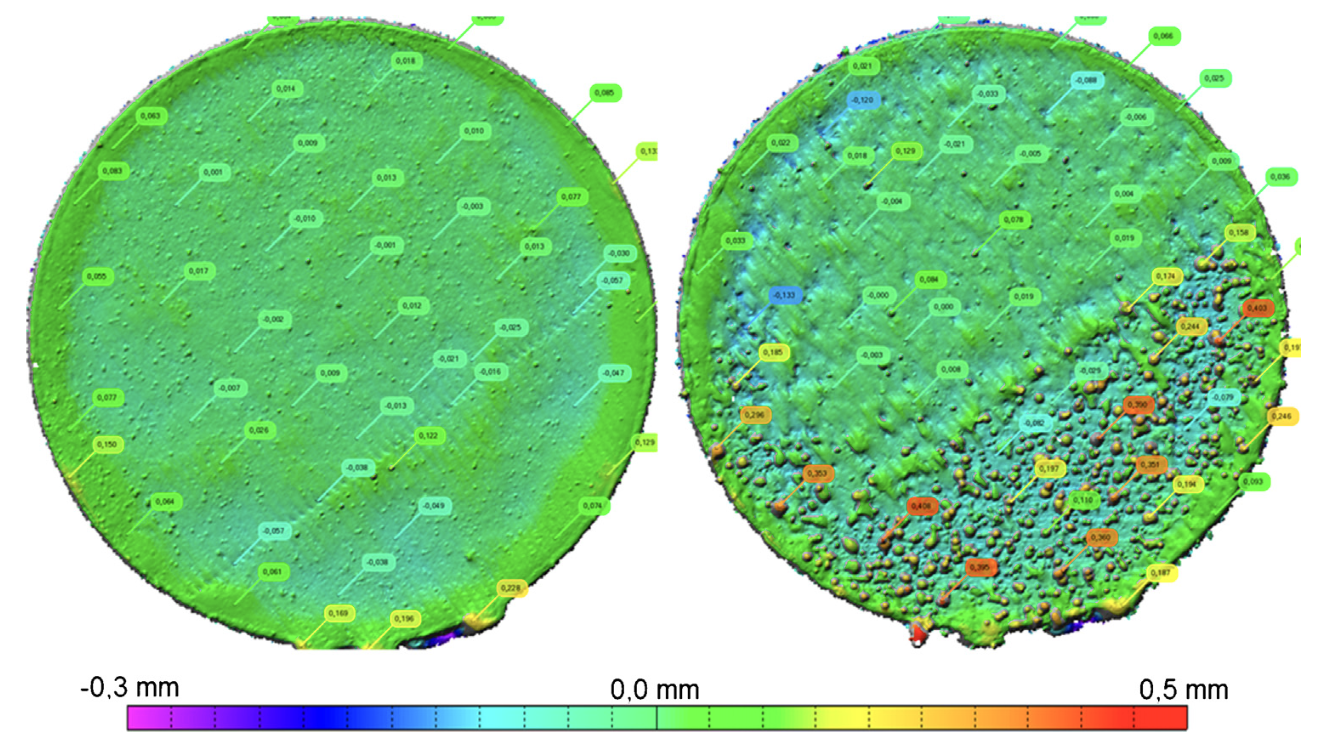
\includegraphics[scale=0.4]{Images/surface.png}
    }
    \caption[Examples of defect in PBF.]{Example of geometrical errors in SLS caused by a wrong support (a) \cite{grasso_-process_2017}, examples of two local oxide contaminations indicated by the red arrows in the fracture surface of an AISI 316L specimen in SLS (b) \cite{casati_microstructure_2016},  good (left) and poor (right) surface textures measured via confocal microscopy on parts produced either in the presence of good and improper gas flow conditions in L-PBF (c) \cite{ladewig_influence_2016}.}
\end{figure} 
\paragraph{Surface defects.} In PBF methodologies, as in most of AM processes, the texture of the surface is influenced by the layer-by-layer manufacturing process, and by the existence of surface impurities, inconsistencies, and voids. The surface's texture is determined by processing conditions, the perimeter scanning technique, and the dimensions of powder particles. The orientation of the surface in relation to building direction influences its texture. In particular, downward-facing and upward-facing surfaces are known to have considerably different texture properties. Even though many parts produced via PBF are refined by post-processing operations (like surface polish and thermal procedures), the texture of the surface is of functional importance since it impacts the part's fatigue resilience. Furthermore, for medical lattice structures, the texture of the surface is can help implant's assimilation during bone healing. Fig. \ref{fig:surface} displays instances of optimal (left) and poor (right) surface textures as observed through con-focal microscopy on components made under optimal and improper gas flow situations in L-PBF \cite{ladewig_influence_2016}. Surface imperfections are further increased by the previously mentioned balling phenomenon, leading to less smooth surfaces.
\paragraph{Microstructural inhomogeneities and impurities.}


% <<< End of Categories of Defect in PBF Processes

%%%%%
%%%%%

% Temperature Anomalies and Hot Spots>>>
\section{Temperature Anomalies and Hot Spots}
\label{sec:hotspot}
As discussed in \citeauthor{williams_situ_2019} (2019), almost all major quality characteristics of the final part and its mechanical performance depend on the thermal history. A specific defect characterized by anomalous temperature profiles is known as hot spot (HS). The primary cause of these defects is the laser beam being repeatedly focused on thermally insulated regions. These are areas predominantly surrounded by powder and lacking any support structure to ensure the proper cooling down phase, as explained in Section \ref{sec:pbf_proc}, but also overhanging walls and sharp edges. This would result in a very localized overheating of the powder bed, leading to the following defects \cite{bugatti_towards_2022}:
\begin{itemize}
    \item \textbf{High surface roughness:} overheated areas can lead to melting unwanted areas of powder and partially melted powder particles attach to the surface. This will result into small melted powder on th surface of the final object, thus increasing its roughness;
    \item \textbf{Change in microstructure of the material:} normal melting zone are characterized by a high cooling rate that leads to finer grain formation, while overheating regions tend to develop a coarser microstructure due to the slower cooling transient;
    \item \textbf{Porosity formation:} if the region is already hot, new laser scans may lead to material vaporization, hence unstable keyhole formation which is often correlated with porosity defects.
\end{itemize} An example of these defects can be seen in Fig. \ref{fig:cane}.

\begin{figure}
    \centering
    \subfloat[\label{fig:dio}]{
        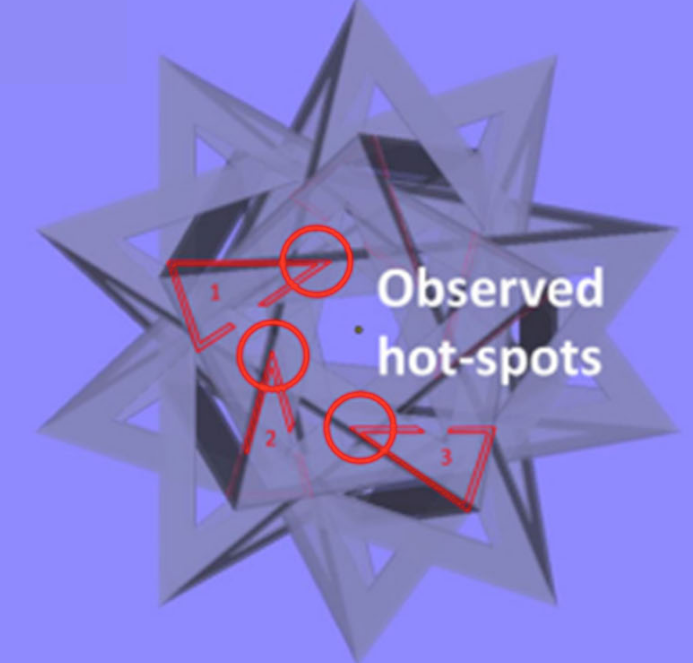
\includegraphics[scale=0.5]{Images/modehs.png}
    }
    \qquad
    \subfloat[\label{fig:cane}]{
        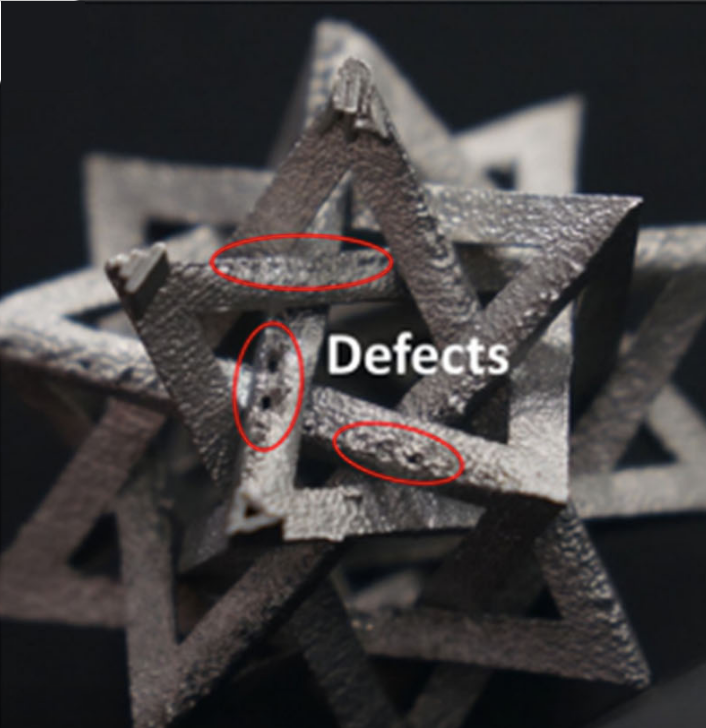
\includegraphics[scale=0.4]{Images/printedhs.png}
    }
    \caption[Examples of hot spot defects.]{Examples of a complex shape CAD model with the position of observed hot spot (a) and relative observed defects in printed part (b) \cite{grasso_-process_2017}.}
\end{figure}
% <<< End of Temperature Anomalies and Hot Spots

%%%%%
%%%%%

% >>> Defects Monitoring Methods
\section{Defects Monitoring Methods}
\label{sec:comelotrovo}
In last years, thanks to advancements in both computational power available at lower cost and rising technology of sensors, quality control has evolved into an increasingly complex and sophisticated process. This is particularly evident in AM (Additive Manufacturing), where we can employ the layer-wise production logic to gather vast amounts of data with remarkable granularity. The aim of this section is to outline the various approaches to quality control, providing a terminology framework as established in \citeauthor{richard_leach_integrated_2020} (2020) and in \citeauthor{grasso_-situ_2021} (2021).

\begin{figure}
    \centering
    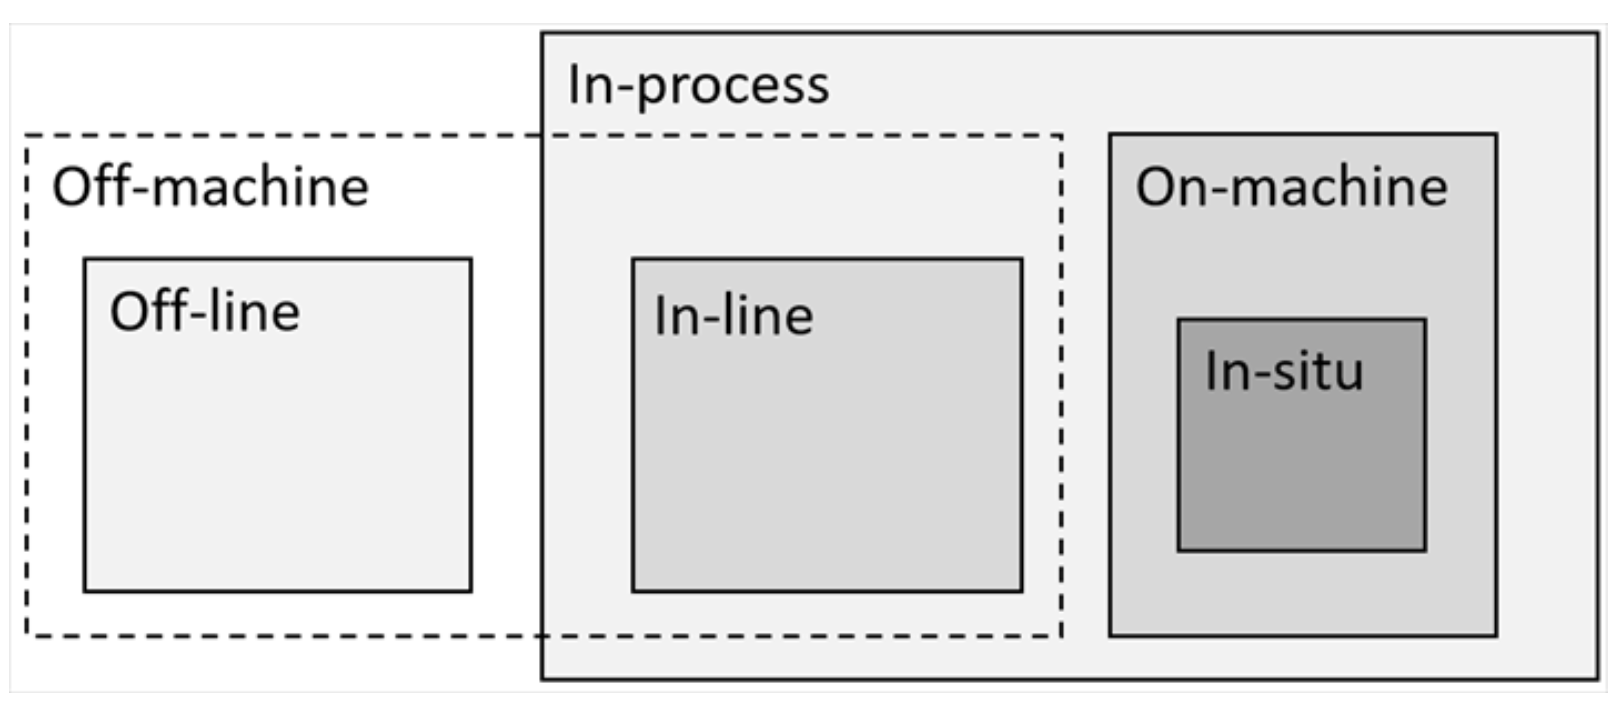
\includegraphics[width=0.6\textwidth]{Images/dovevai.png}
    \caption[Measurement and monitoring techniques.]{Graphical representation of different terms associated with measurement and monitoring techniques \cite{richard_leach_integrated_2020}.}
    \label{fig:dovevai}
\end{figure}
\emph{In-process} methods involve the measurements of any data during the process or between consecutive production phases within the same manufacturing chain. These measurements are syncronized with the different stages of the manufacturing process, thus allowing monitoring it in a synergistic way. When in-process measurements are executed immediately before, after, or amidst manufacturing points, they're called \emph{"in-line"} measurements. These are captured on distinct measurement systems along the standard production line, where manufacturing is not occurring. Consequently, they fall under 'off-machine' measurements. \emph{off-machine} measurements are taken outside the machine where the manufacturing process occurs. Conversely, if measurements taken during the process use sensors mounted on the production machine, they're labeled \emph{'on-machine'} measurements. Those that principally document data directly from the manufacturing site are called "in-situ" measurements. In AM processes, \emph{in-situ} predominantly denotes sensing and surveillance techniques aiming to capture details about process stability and product caliber during the manufacturing process. Data collected from this last method are particularly significant as they are gathered very close to the final product and are carrying a lot of information. Conversely, when the metrics aren't "in-process", they're labeled as \emph{"off-line"} or \emph{"ex-situ"}. They're categorized as off-machine measurements since they're usually executed outside the core manufacturing setup, perhaps at a separate factory measurement station or a lab. Within the domain of in-situ measurements, there is a small difference between 'in-situ measurement' and 'in-situ monitoring'. The former implies the capability of in-situ sensors to gauge aspects, aiming to understand the process or assess the product's quality attributes during production. The latter alludes to the real-time identification of discrepancies, abnormalities, and unregulated process conditions potentially inducing product flaws, often requiring the establishment of an alert system or classification algorithm. 
Furthermore, considering "in-situ" measurements, depending on the signature of the process being measured, we can distinguish five different levels of monitoring \cite{grasso_-situ_2021, grasso_process_2017}. These levels are referred to "observable signatures" only, i.e. measurable quantity, while the "derived signatures", i.e. quantitis estimated via process modelling, are included in the process modelling literature.  Let's delve into the specifics of measurements levels, which are represented in Fig. \ref{fig:levels}.
\begin{figure}
    \centering
    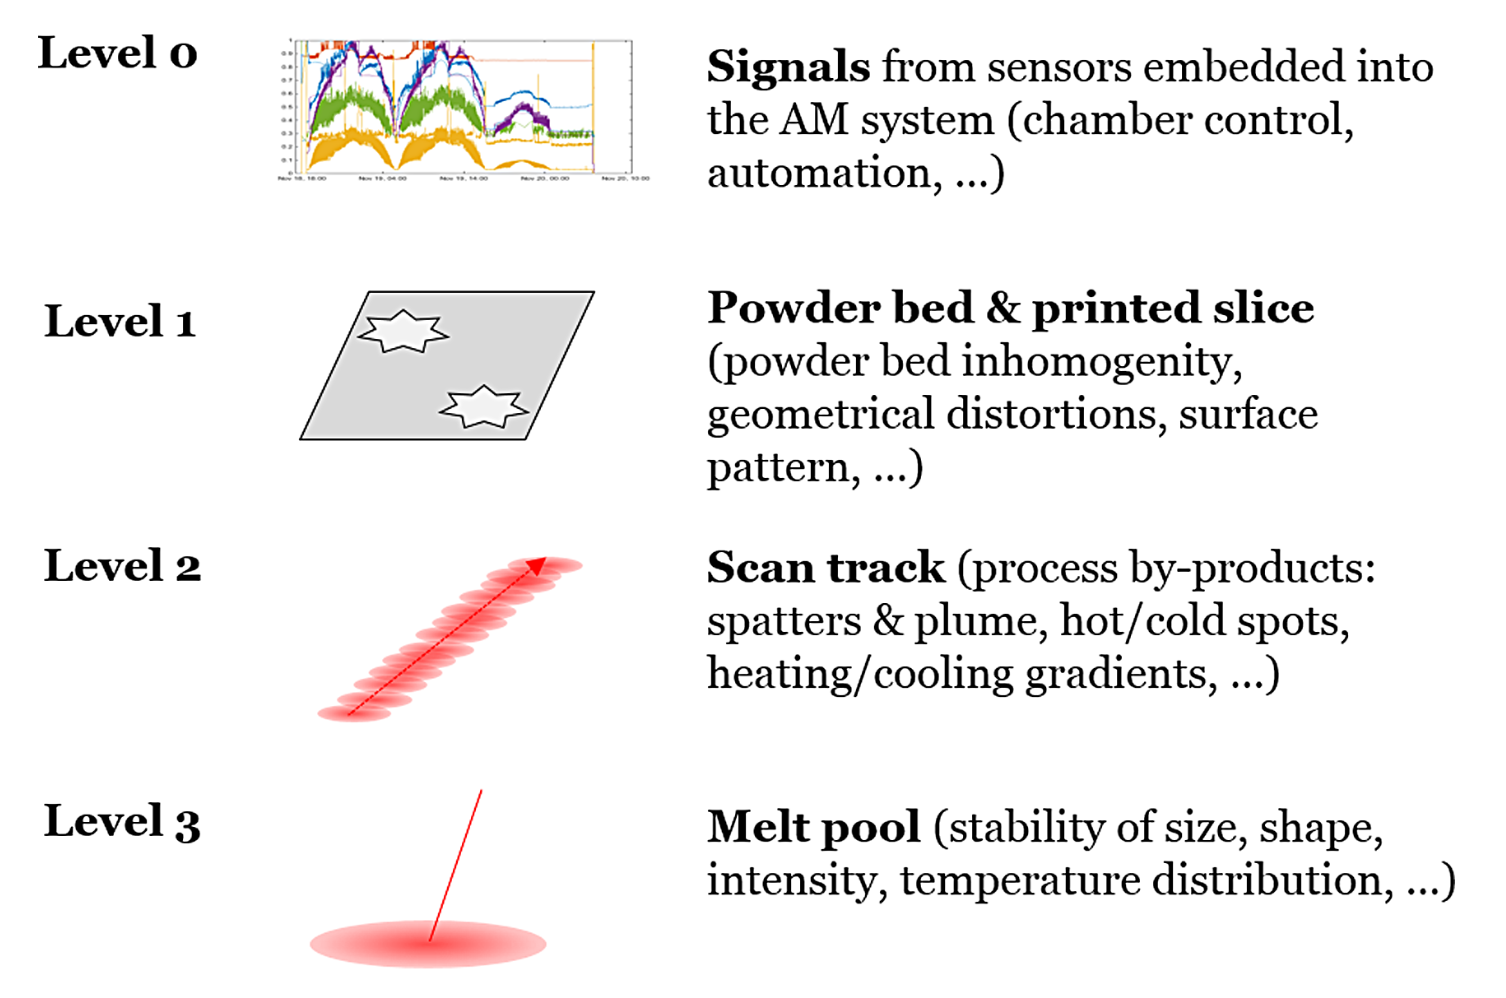
\includegraphics[width=0.6\textwidth]{Images/Level Measurement.png}
    \caption[In-situ measurement levels.]{Five in-situ measurement levels applicable to PBF processes \cite{leach_-machine_2020}.}
    \label{fig:levels}
\end{figure}

\begin{enumerate}
    \item \textbf{Level 0:} in this level we lever all the signals that can be measured using embedded sensor to detect anomalies and unstable processes state. Apart from defects detection purposes, usually these signals are employed to keep the machine state and the machine chamber environment under control. Some examples of these signals are chamber pressure, ambient temperature and inert gas flow;
    \item \textbf{Level 1:} this level involves measurements gathere once (or more than once) per layer of the entire build area. In this level we are interested in both the homogeinity of the powder bed and the geometrical and dimensional feature of the printed slice;
    \item \textbf{Level 2:} this level includes quantities that can be measured with temporal resolution. Usually, this temporal resolution is higher than the layer-wise resolution in previous level;
    \item \textbf{Level 3:} it encompasses the evaluation of process signatures with the higher granularity possible in PBF systems, i.e. the melt pool. 
    \item \textbf{Level 4:} this level regards the capability of gathering information about phenomena occurring under the currently processed layer. These measurements can be obtained with adhoc prototype machine configurations that enable transverse x-ray imaging, but also ultrasound and acoustic emissions caused by the release of elastic energy and plastic deformation of solidified layers.
\end{enumerate}
% <<< End of Defect Monitoring Methods


% >>> Sensors for anomalies detection
\section{Sensors for Anomalies Detection}
\label{sec:sensoriniiniini}
Each level described in Section \ref{sec:comelotrovo} involves different sensor tipologies. In this section I will provide a description of the most widely used sensors in in-situ proccess monitoring and measurement in AM. 
In \emph{level ~0}, we can use embedded sensors integrated within the printer, the same sensors that the printing control unit uses to adjust printing parameters. However, publications proposed a more advanced in-process use of signals from such sensors only in EB-PBF applications as a possible source of information for in-situ anomaly detection as in \citeauthor{grasso_data_2018} (2018) and \citeauthor{steed_falcon_2017} (2017). Same publications pointed out that many of these EB-PBF log signals are correlated with process errors and variations in process conditions. EBM Embedded sensor signals in EB-PBF are also known as ‘log signals’. \citeauthor{steed_falcon_2017} (2017) proposed a software tool for visualisation and analysis of large multivariate time series log signals called Falcon. In \emph{level ~1}, i.e. measurement and characterisation of layer properties, we can distinguish two further types of measurements. The first is conducted before laser scanning, which allows us to identify areas where the powder is not uniform, potential defects produced by the recoating system or the so-called super-elevated edges, i.e. areas of the previously printed slice that could not be fully covered by the new powder layer. The second is performed after the laser scanning, through which we can detect any contamination of the powder of the printed slice or any geometric or dimensional deviations from the nominal shape. There are several types of sensors that can be employed for anomaly detection at this level.
\begin{figure}
    \centering
    \subfloat[\label{fig:offaxiallaser}]{
        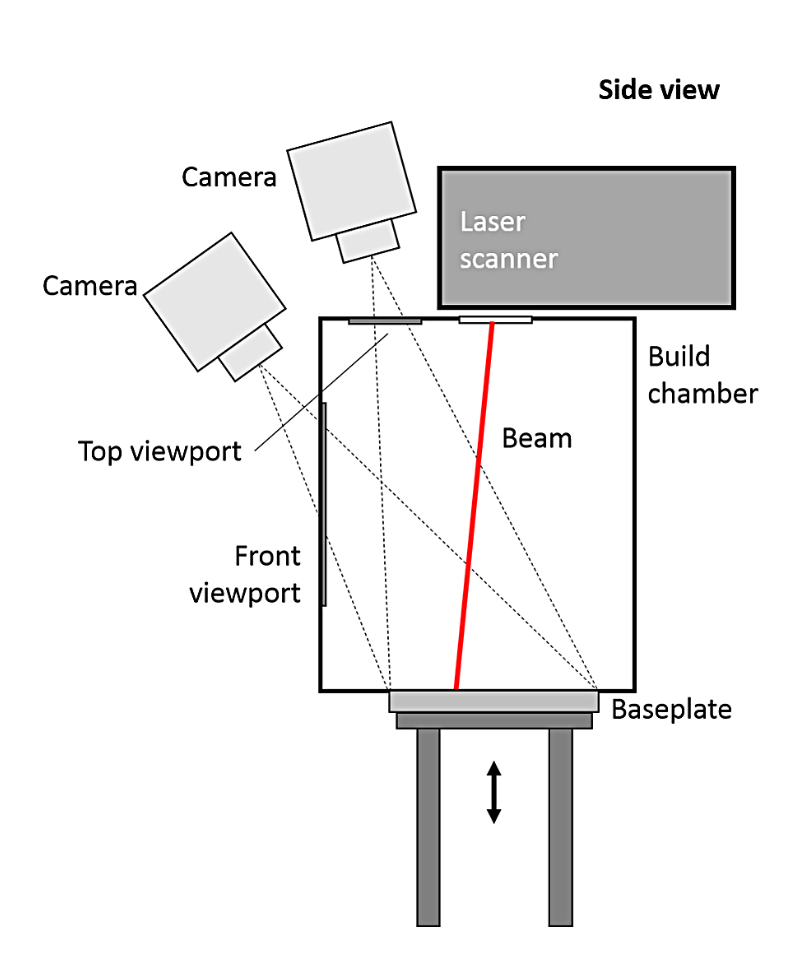
\includegraphics[scale=0.35]{Images/off axial laser.png}
    }
    \qquad
    \subfloat[\label{fig:fig:offaxialebm}]{
        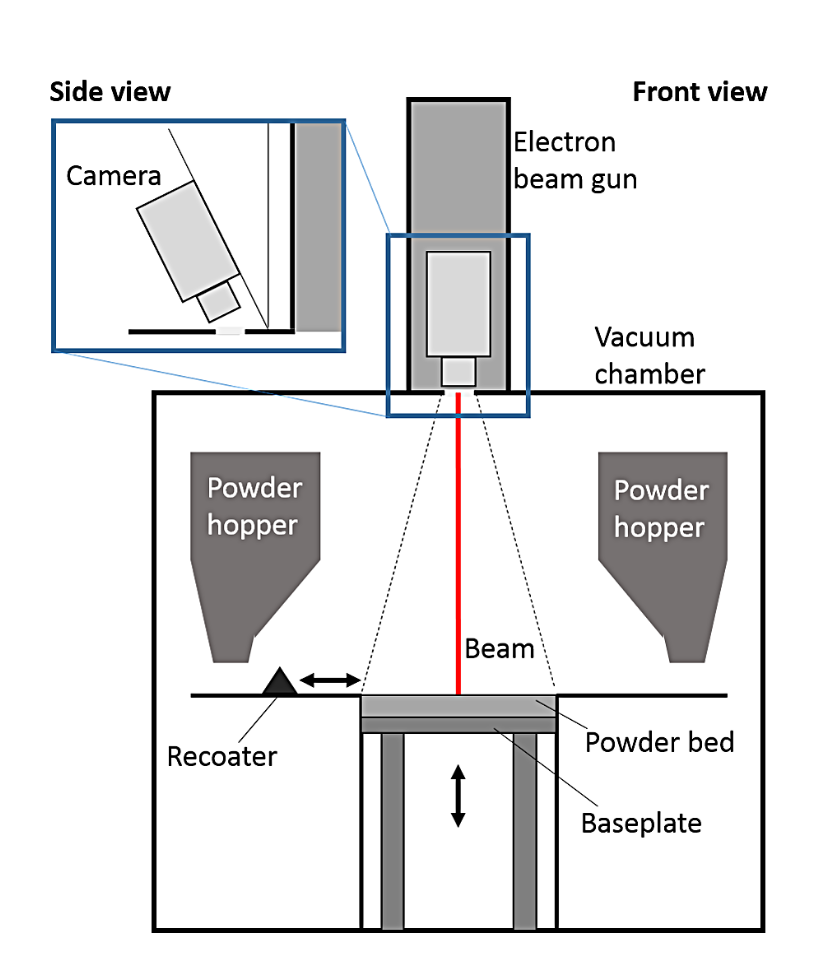
\includegraphics[scale=0.35]{Images/off axial EBM.png}
    }
    \caption[Off-axis sensing.]{Example of off-axis sensing architectures in SLS (a) and EBM (b) \cite{leach_-machine_2020}.}
\end{figure}
\paragraph{Off-Axis Sensing.} In both SLS and EBM, off-axis sensing is suitable to gather information. Conventional camera operating in the visible range are usually employed in L-PBF (Fig. \ref{fig:offaxiallaser}), while the high temperatures in EBM recoating and the difficulty to install additional sensors on EB-PBF machines (Fig. \ref{fig:fig:offaxialebm}), makes their usage more challenging. The off-axis optical camera within the visible range, however, has a significant drawback: numerous publications as \citealt{kleszczynski_error_2012} (2012) and \citeauthor{foster_bk_optical_2015} (2015) have shown how appropriate illumination condition greatly impacts the camera's acquired result. Both the surface pattern of the printed slice and the powder bed, as well as the contrast between the background (powder) and foreground (printed slice) areas, are influenced by the intensity, nature, and relative angle of the illumination source. Non-uniform illumination conditions may mask some anomalies. The relative angle between the camera and the illumination source also plays a relevant role in this kind of measurement as shown in  \citeauthor{caltanissetta_characterization_2018} (2018). Moreover, the distorted perspective given by the camera's positioning needs to be corrected through specific geometric adjustment operations before analysis. In addition to traditional cameras, those operating in the NIR/IR range can also be used in process monitoring of level 1 process signatures. They prove particularly valuable in EBM processes due to the high temperatures encountered during the printing process. Two examples of acquired images can be seen in Fig. \ref{fig:quadratoir} and Fig. \ref{fig:cilindroir}
\begin{figure}
    \centering
    \subfloat[\label{fig:quadratoir}]{
        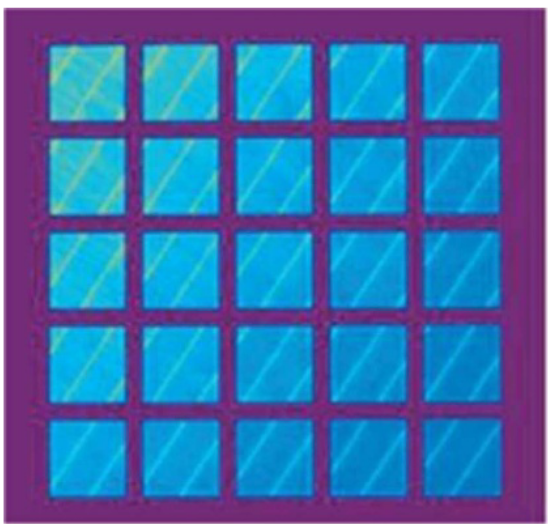
\includegraphics[scale=0.45]{Images/quadratoir.png}
    }
    \qquad
    \subfloat[\label{fig:cilindroir}]{
        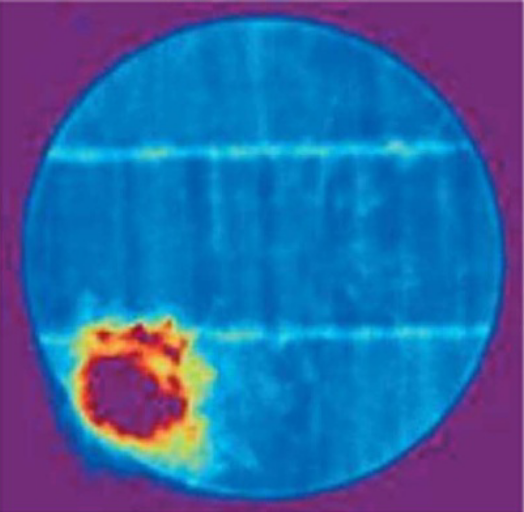
\includegraphics[scale=0.45]{Images/cilindroir.png}
    }
    \caption[optical tomography examples.]{Examples of optical tomography images for cubic samples with variation of energy density (a) and a cylinder produced under shielding gas flow variation (b)\cite{bamberg_-process_2016}.}
\end{figure}
One of the most employed system for this kind of measurement is ‘LayerQam’, developed by Arcam (GE Additive) for integration in its EB-PBF machines. The system consists of a NIR camera that acquires an image of the layer after the melting phase and use local pixel intensity variations. Furthermore, the presence of bright spots are used as proxies of possible volumetric flaws and material discontinuity defects.

\paragraph{Fringe Projection.} The off-axis imaging techniques mentioned in the preceding paragraph can be used for generating a 2D reconstruction of the powder bed and the printed section. With fringe projection, we can achieve a height map of the powder bed. The classic setup A method advocated by several researchers is fringe projection, which merges layer visualization with topographic examination. This method necessitates one or more cameras along with a projector, with diverse setups being suggested in scholarly articles, primarily for L-PBF. The standard configuration for such measurements consists of a camera (single view configuration) and a projector. The graphic representation of the system can be seen in Fig. \ref{fig:fringesetup}, while in Fig. \ref{fig:fringeprojection} there is an example of an height map.
\begin{figure}
    \centering
    \subfloat[\label{fig:fringesetup}]{
        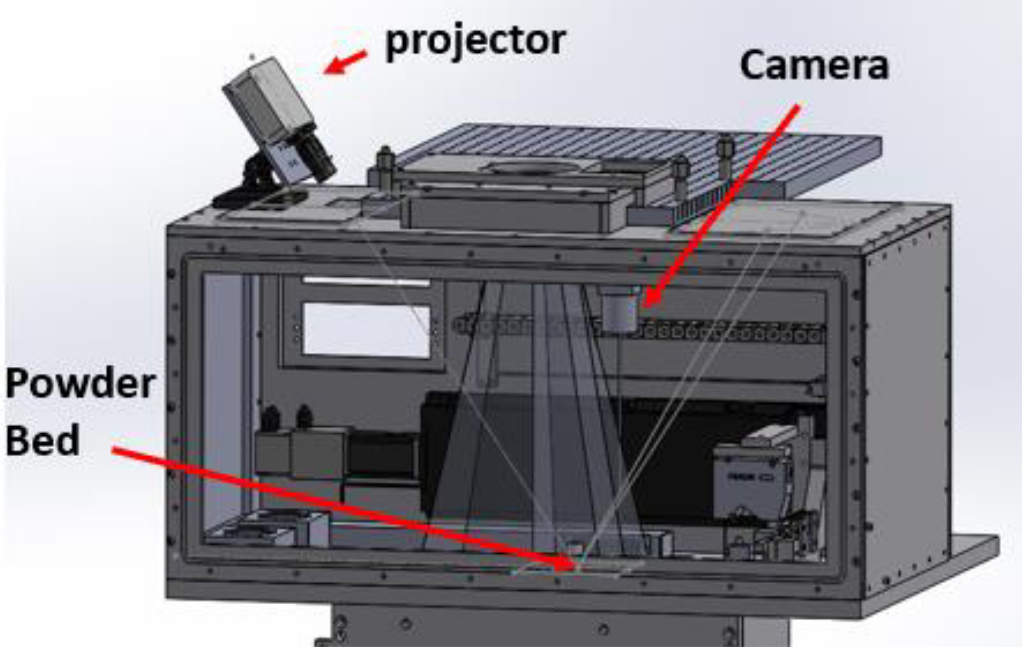
\includegraphics[scale=0.35]{Images/fringesetup.png}
    }
    \qquad
    \subfloat[\label{fig:fringeprojection}]{
        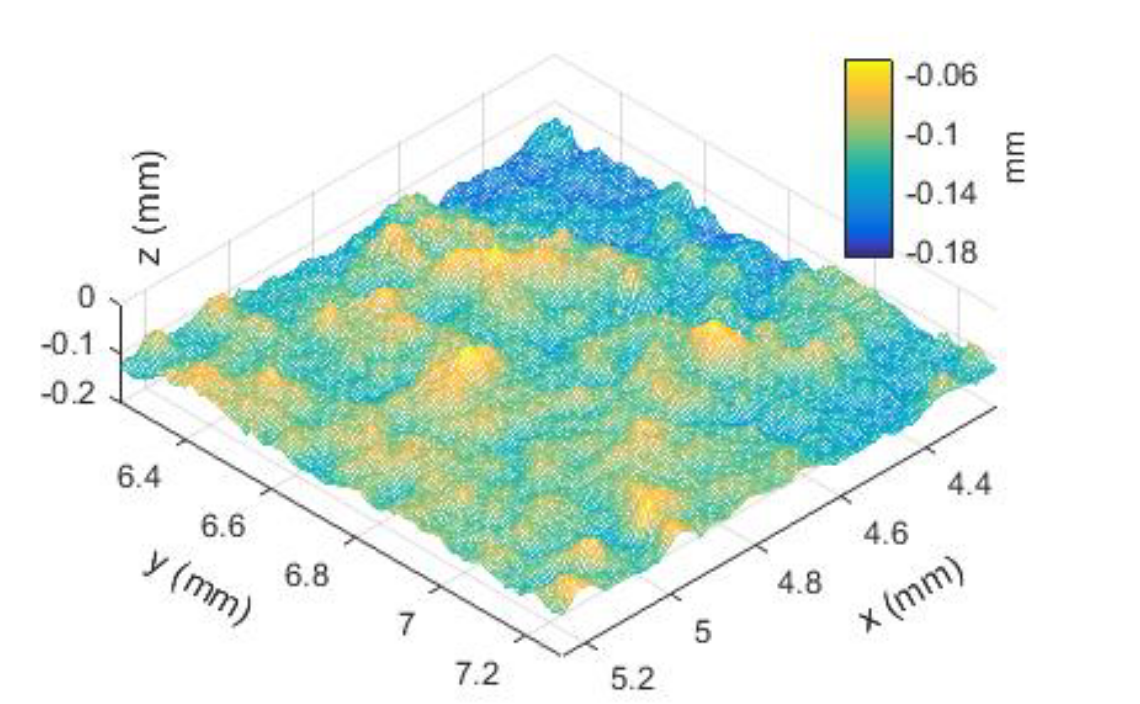
\includegraphics[scale=0.35]{Images/fringeprojection.png}
    }
    \caption[Fringe projection.]{Setup for fringe projection measurement system (a) and reconstructed height map of the power bed (b) \cite{zhang_situ_2016}.}
\end{figure}
Other authors proposed and tested multi-view configurations, with two or more cameras, suitable to achieve higher resolution and accuracy, like in \citeauthor{kalms_new_2019} (2019).
\paragraph{Blade Mounted Sensor.} Another possible approach for level 1 process monitoring is to employ an optical sensor directly mounted on the recoating blade of PBF printers. In this way, we can eliminate the geometric distortion typical of off-axis systems. Moreover, these sensors can be used both for obtaining a 2D representation of the print bed and for reconstructing the height maps. In the former case, we can obtain a resolution up to \SI{4800}{DPI} over a length of \SI{210}{\milli\metre} with a spatial resolution of \SI{5.3}{\micro\metre / pixel} \cite{tan_phuc_high-resolution_2019}, while in the latter with a little lower resolution of \SI{20}{\micro\metre / pixel} \cite{barrett_micron-level_2018}.

\paragraph{Co-axial sensing.} L-PBF offers the possibility to leverage the back-scattered light from the melt pool and its adjacent areas, to gauge specific metrics indicative of melt-pool dynamics. Scattered light pass through the optical path of the laser, passing the same lenses of processing laser, and a semi-reflective mirror redirects the laser beam to the scanner, while simultaneously allowing the light emitted from the melt pool to be detected by sensors. This emitted light is then divided and directed to each sensor. Various co-axial detection designs might encompass multiple pyrometers, bi-wavelength or multi-wavelength pyrometers, and assorted imaging devices in either the visible or infrared spectrum. An example of a co-axial sensing system can be seen in Fig. \ref{fig:coaxiallaser}. With this method, we can reach really high sample rates of \SI{50}{\kilo\hertz}, but the observation area is typically limited to \SI{0.5}{\milli\metre} $\times$ \SI{0.5}{\milli\metre}, making this method unsuitable to capture time evolution. Alterations in the melt pool's dimensions and luminosity/temperature can induce changes in the pyrometer's readings, facilitating the observation of melt pool consistency and any unusual signal shifts. This architecture was first developed by the Katholieke Universiteit Leuven and licensed by Concept Laser \cite{leach_-machine_2020, kruth_jean-pierre_feedback_2007, berumen_quality_2010}. This measurement approach has achieved outstanding results, with a lateral resolution of \SI{30}{\micro\metre} and a vertical resolution of \SI{7}{\micro\metre} truly impressive lateral and vertical resolutions: the former being 30 micrometers and the latter at 7 micrometers \cite{fleming_tracking_2020}.
\begin{figure}
    \centering
    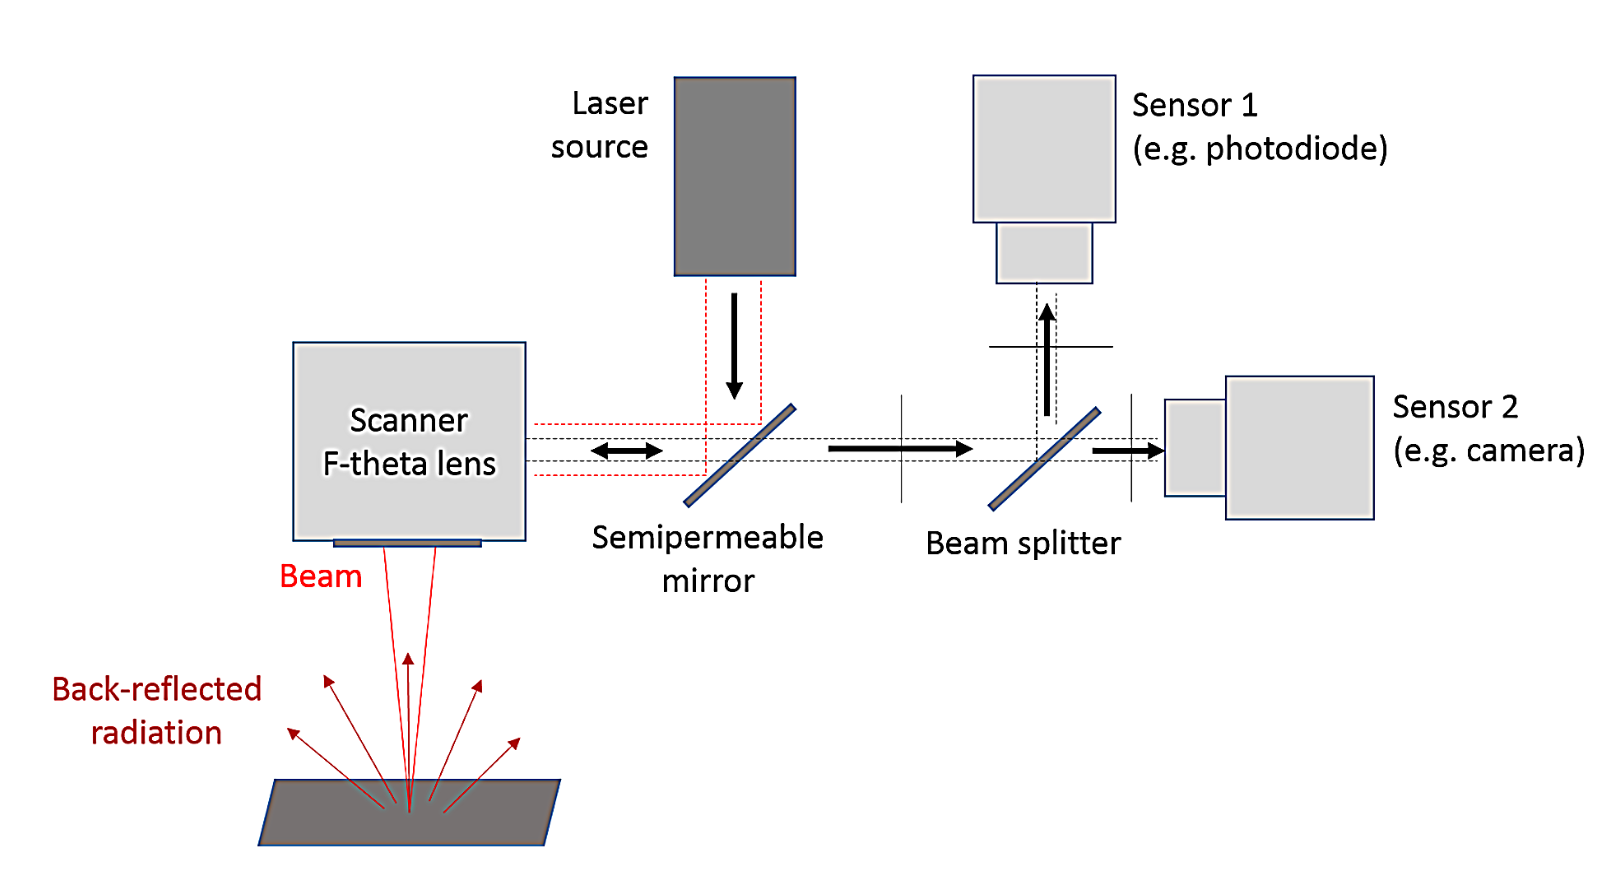
\includegraphics[width = 0.6\textwidth]{Images/coaxial laser.png}
    \caption[Co-axial sensing system.]{A graphical representation of a system for co-axial sensing in L-PBF \cite{leach_-machine_2020}.}
    \label{fig:coaxiallaser}
\end{figure}


\begin{figure}
    \centering
    \subfloat[\label{fig:coaxialROI}]{
        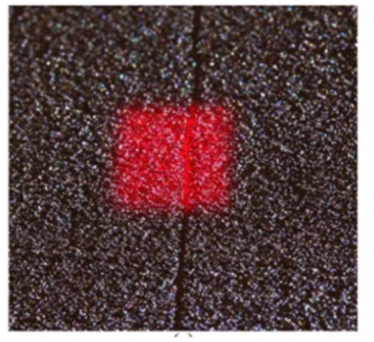
\includegraphics[scale=0.5]{Images/coaxialROI.png}
    }
    \qquad
    \subfloat[\label{fig:coaxialheatmap}]{
        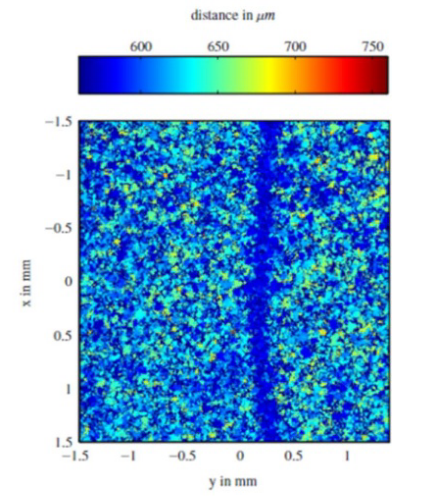
\includegraphics[scale=0.55]{Images/coaxialmap.png}
    }
    \caption[Co-axial sensing result.]{Region of interest covered by co-axial imaging (a) and corresponding in-situ topography reconstruction (b) \cite{neef_low_2014}.}
\end{figure}
\paragraph{Electronic imaging.} In EBM, the process gives rise to by-products like secondary and backscattered electrons, as well as x-rays. The electrons generated from the interaction between the beam and metal powder could be harnessed could be used to produce an electronic representation of the layer. Thus, one of the undesired effects outlined in Section \ref{sssec:electroninteractions} can be levered to extract valuable insights about the current state of the process. Using only back-scattered electrons electrons, \citeauthor{wong_pilot_2019} were able to reach a spatial resolution of \SI{60}{\micro\metre / pixel}, we can see an example in Fig. \ref{fig:electronic1}. Moreover, we can use electron beam to scan the layers and metal surfaces, using the heat shield as an electron collector also during the melting phase as done by \citeauthor{arnold_operando_2020}, thus it is a real-time measurement. This approach lead to a resolution of \SIrange[range-phrase=--]{50}{100}{\micro\metre / pixel}. An image from the study can be seen in Fig. \ref{fig:electronic2}.

\begin{figure}
    \centering
    \subfloat[\label{fig:electronic1}]{
        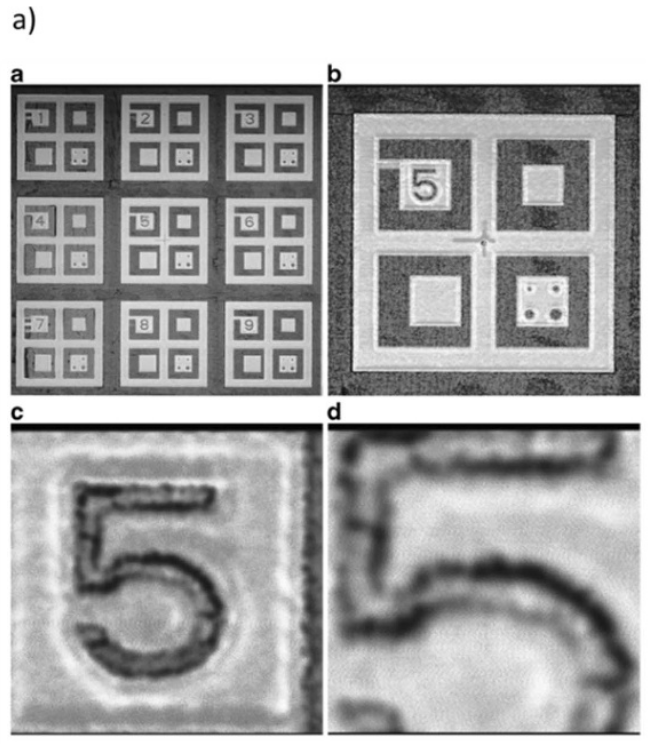
\includegraphics[scale=0.44]{Images/electronic1.png}
    }
    \qquad
    \subfloat[\label{fig:electronic2}]{
        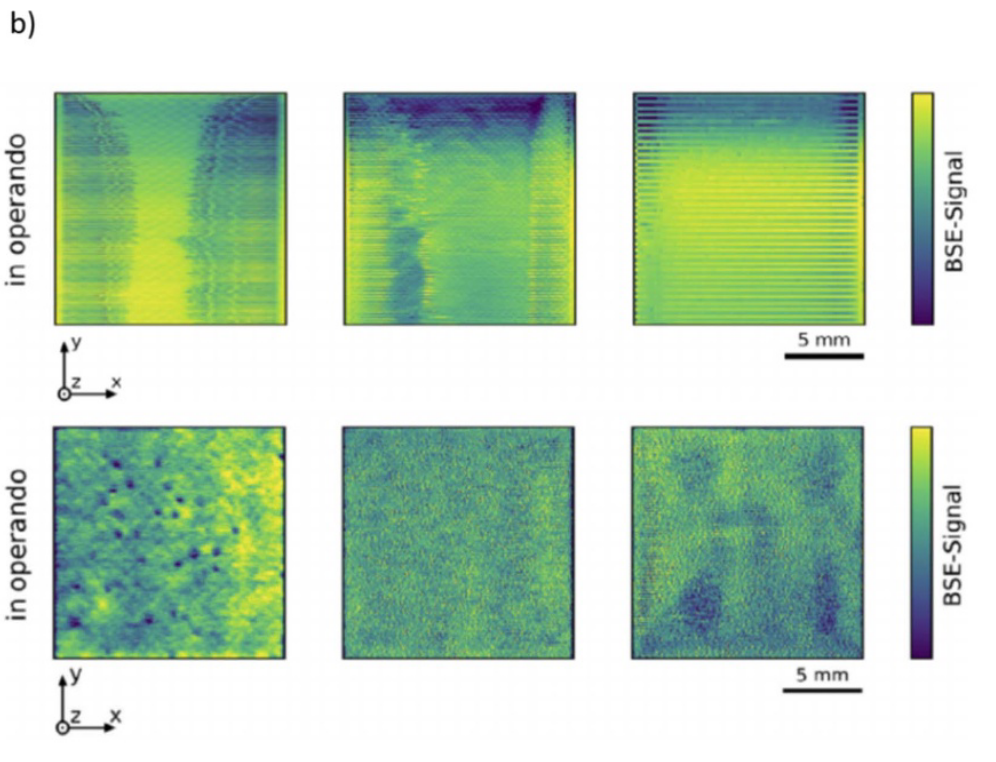
\includegraphics[scale=0.5]{Images/electronic2.png}
    }
    \caption[Co-axial sensing result.]{Examples of electronic images in EBM: images with different magnification factors (a) \cite{wong_pilot_2019} and images of squared printed areas generated via real-time back-scattered signal acquisition from different materials and with increasing hatch spacing \cite{arnold_operando_2020}.}
\end{figure}
For \emph{level ~2} process signatures, we use sensors for in-process measurement of fast transient phenomena and high-speed emissions during laser or electron beam scanning. The main goals of this level is to understand underlying physical phenomena which lead to the formation of the defect. Most of the methods used in this level involve off-axis mounted sensors, mainly cameras in the visible range or thermal cameras with really high temporal resolution. Indeed, this is needed to capture fast and transient phenomena. There are different research streams.



\paragraph{Measurement of Process Heatmap and Temperature Profiles.} We will address this paragraph with greater detail as as these are the methods used to detect the defects discussed in Section \ref{sec:hotspot} and it will be usefull to understand the new proposed method in Chapter \ref{ch:baggingvoronoi}. 
\begin{figure}
    \centering
    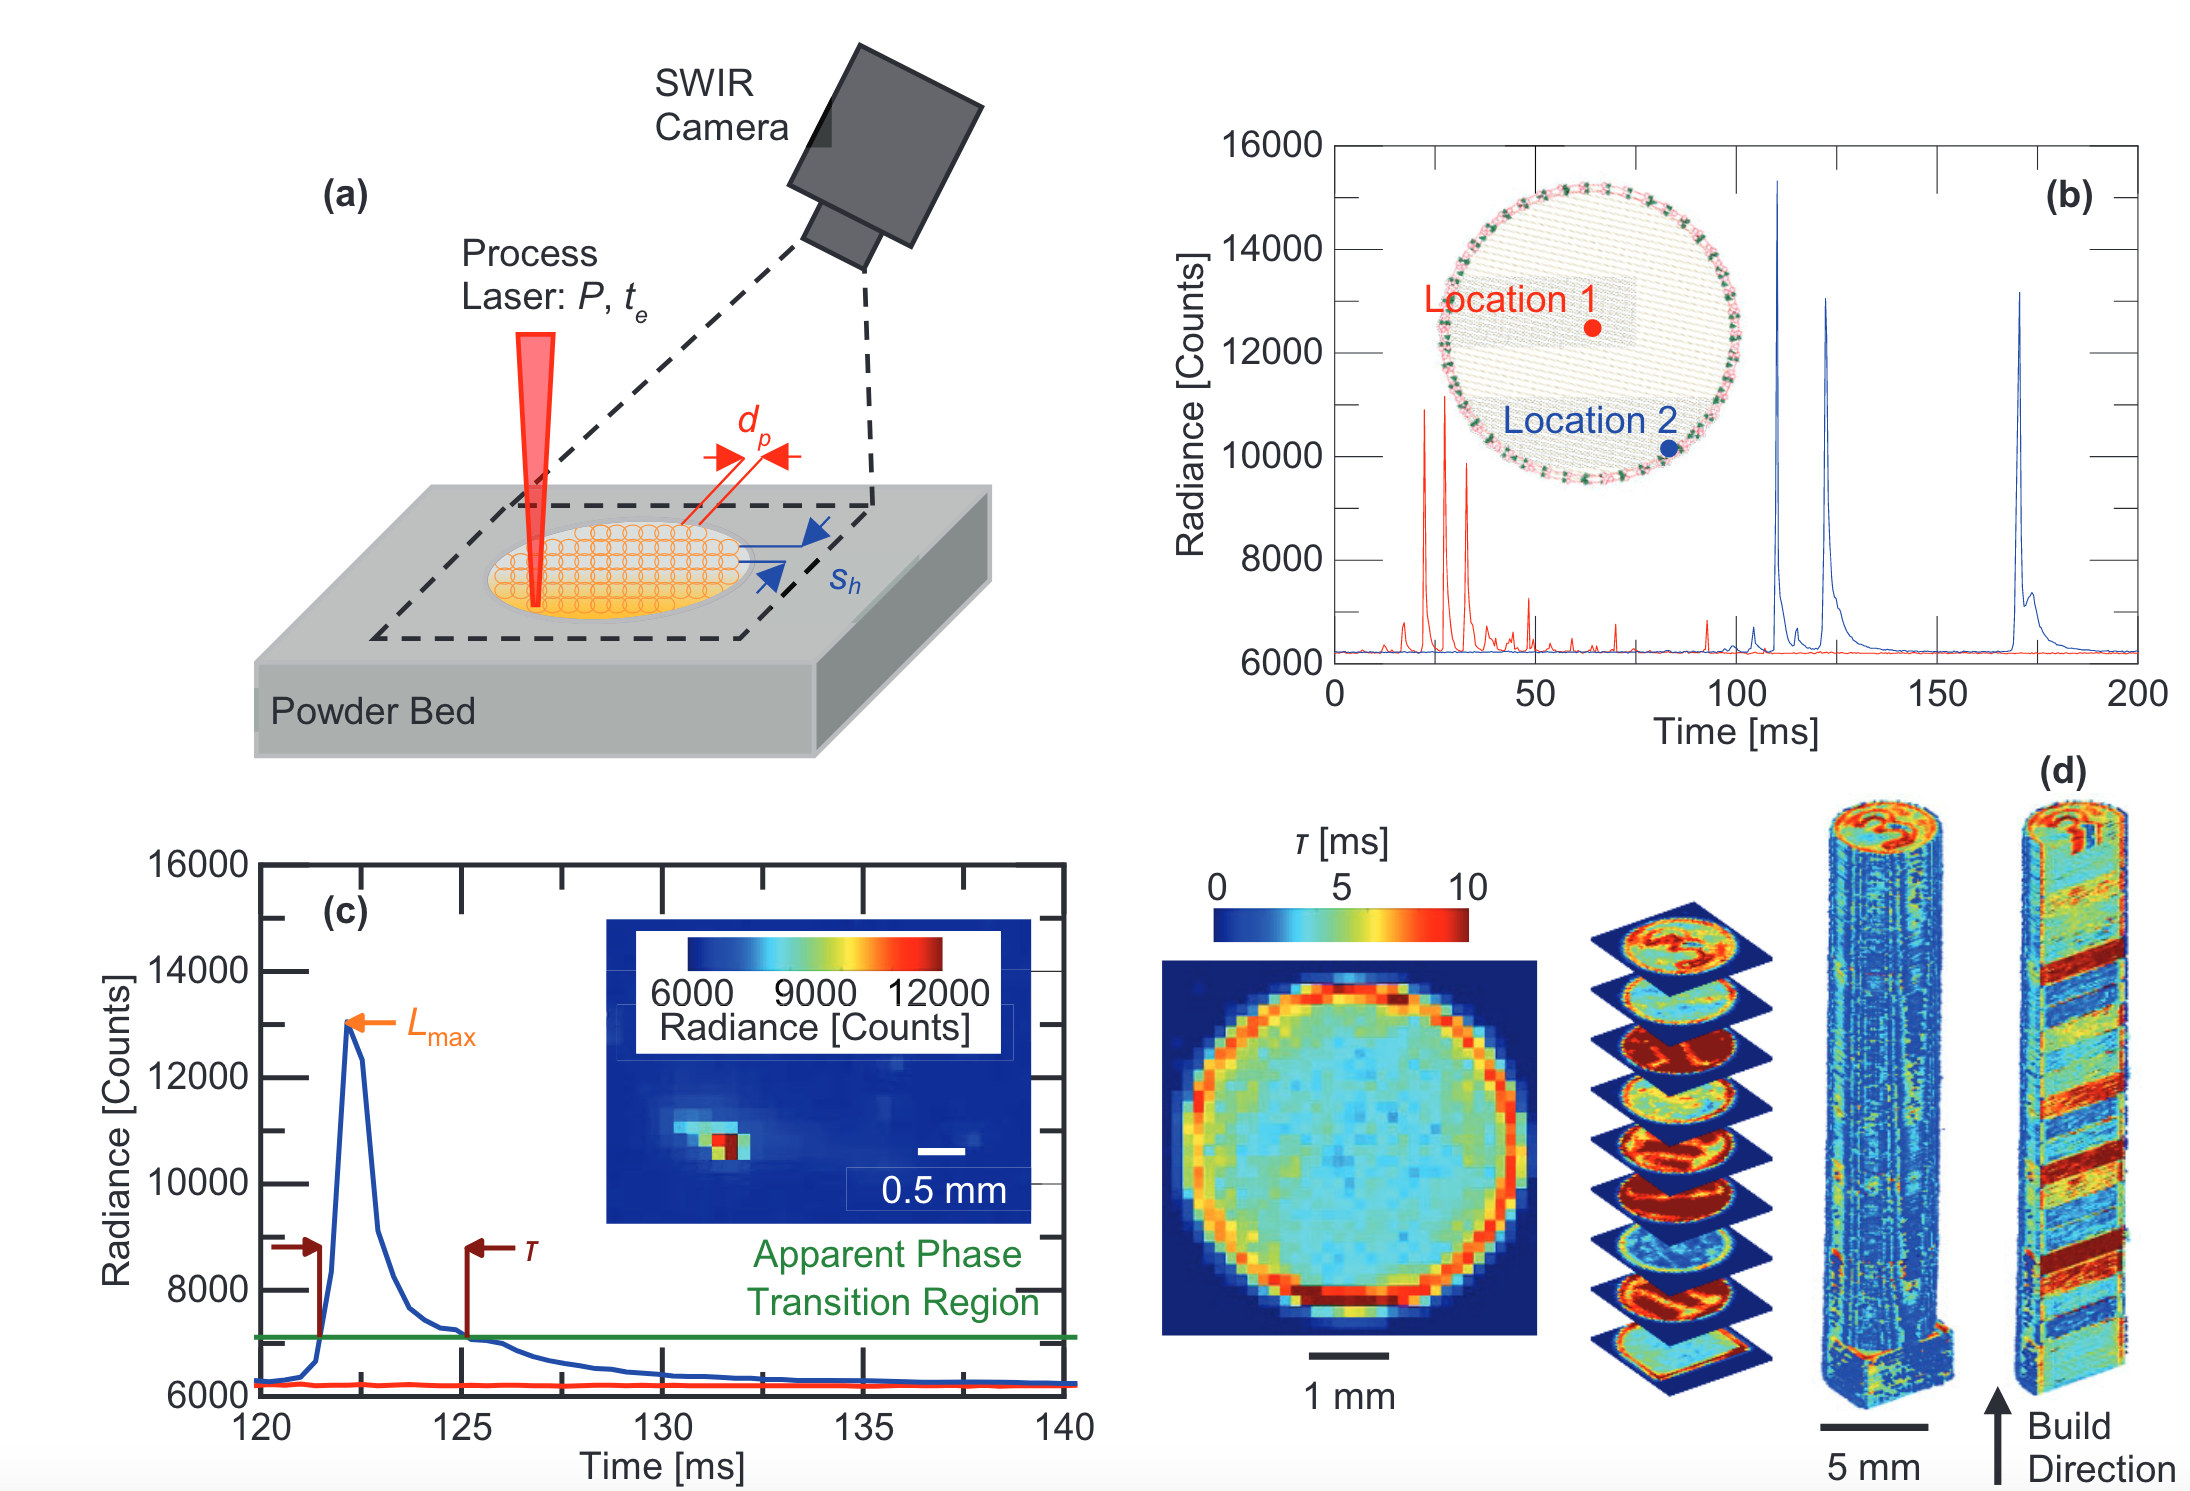
\includegraphics[width=0.8\textwidth]{Images/voxel.png}
    \caption[Example of voxel thermic reconstruction.]{(a) SWIR camera observation of SLM process, (b) time series data from location in center of part cross-section (location 1) and border scan region (location 2), (c) definition of thermal features in time series data with melt pool image, and (d) thermal feature maps showing generation of volumetric data and slicing \cite{lough_-situ_2019}.}
    \label{fig:voxel}
\end{figure}
The layerwise manufacturing paradigm allows the ‘seeing’ of the thermal history of the process, in a new dual-paradigm. In this new paradigm, time and space overlaps over the z-axis. Indeed, the production of an object using additive manufacturing grows in the same direction over time and space. We have already discussed in Section \ref{sec:hotspot} that almost all major quality characteristics of the final part and its mechanical performance depend on the thermal history. Local and global variations of heating and cooling patterns may indicate either LoF or an HS with resultant effects on material solidification at volumetric, microstructural and geometrical levels. We can identify two primary goals linkted to this monitoring system. One focuses on building a heatmap of the layer using data collected at slower rates (up to 50 fps), and the other targets recording rapid thermal fluctuations, with time resolutions ranging from 300 fps to over 10,000 fps. In term of spatial resolution, we can use measurement setups with a limited field of view, which enable us to reach a resolution of \SIrange{8}{100}{\micro\metre / pixel}, of with a field of view covering the entire build area, with a resolution typicalli above \SI{100}{\micro\metre / pixel}. In both L-PBF and EBM we can use thermal cameras, either in the short, medium or long wave IR. To minimize measurement errors caused by the laser's light emissions, one should opt for a short wave IR camera, with a band-width from \SIrange{1.35}{1.6}{\micro\metre} \cite{heigel_situ_2020}. Using this type of camera, the authors were able to produce a thermal map of a specimen printed with L-PBF. Subsequently, by utilizing the features extracted from this map, they achieved a voxel-based representation of the part, associated with its local and global quality attributes. In Fig. \ref{fig:voxel} there is the recostruction of the specimen. Although they exhibit a heightened sensitivity to emissivity values when determining absolute temperatures, thermal cameras in the medium or long wave IR spectrum can be adjusted over a broader temperature span compared to short wave IR cameras. They maintain high sensitivity even at elevated temperatures, which has made them the preferred sensors for in-situ thermal video imaging in both L-PBF and EB-PBF applications, especially when we need a larger field of view to construct thermal map.  Other researchers have employed high temporal resolution IR video imaging in L-PBF to improve the ability to map temperature profiles spatially and temporally, also capturing quick and transient events. In EB-PBF, the methodologies for in-situ video imaging have to be tailored to cater to the unique aspects of the process. Both standard and thermal imaging devices must shield against x-ray emissions and metal deposition. With this in mind, existing viewports can be outfitted with x-ray shielding glass and a rotating Kapton film, ensuring that metallic vapours don't settle on the glass. The Kapton film allows for approximately 79\% IR transmission, while a 10 mm x-ray shielding window lets through around 1.08\% of IR, as noted by \cite{ralph_b_dinwiddie_thermographic_2013}. Yet, given the elevated temperatures in the procedure, comprehensive IR imaging potential has been demonstrated in studies, even with such diminished transmission rates. Although IR cameras provide precise spatial and temporal readings of thermal shifts, pinpointing exact temperatures proves challenging. PBF processes experience rapid state changes, transitioning from powder to a liquid state and then to a solidified form. This, combined with ongoing alterations in surface attributes and vaporized material emissions, constrains the accurate estimation of emissivity essential for converting base signals into temperature measurements. For numerous in-situ monitoring endeavors, the importance lies in the thermal signature's fluctuation over time rather than pinpointing an absolute temperature. In such instances, data analysis and monitoring algorithms can be employed directly on the basic signals, which are the recorded radiance figures in arbitrary metrics. If precise temperature approximations are vital, alternative techniques come into play. While thermal cameras are bulky, costly, and generally call for alterations in machinery hardware and viewports for assimilation into commercial setups, standard cameras are more cost-effective and straightforward to incorporate. With the right equipment, they can offer high temporal precision. Even though they don't grant precise temperature assessments, variations in pixel brightness in the visible spectrum can serve as markers for genuine thermal shifts to spot abnormalities and imperfections in certain scenarios. Within this context, certain research endeavors have zeroed in on identifying localized intense heat events, referred to as 'hot-spots', using rapid video imaging in the visible domain. A hot-spot is characterized by a localized excessive heating of the layer due to unregulated thermal interactions with the nearby matter. An area impacted by a hot-spot remains elevated in temperature (appearing bright) for an extended duration, cooling at a decelerated rate compared to regular scenarios. Hence, a standard camera, equipped with the right temporal capabilities, can effectively detect such irregularities.
\paragraph{Process By-Products Measurement.} Due to the different nature of the interactions in the SLS and EBM processes, as already described in \ref{sec:matterint}, we need to distinguish between the measurement systems of the by-products of these two processes. Since we already discussed the measurement of the by-products of EBM in level 1, in this paragraph we will focus on L-PBF processes. It has been widely demonstrated that the partial vaporization of the metal, also called plume, and the spatter ejected together with it are correlated with detrimental effects on part quality. Indeed, the emissions of these by-products, if too intense, could lead to the deflection and partial absorption of the laser beam, leading to a change in the laser spot geometry or energy density. Fig. \ref{fig:plume} shows a graphical representation of the phenomenon just described. To obtain information about spatter and plume, visible and IR video imaging techniques can be employed. In Fig. \ref{fig:colosimoplume} we can see an example of an in-control plume generation phenomenon acquired using IR camera. Recent research has introduced a high-speed stereo vision system to pinpoint and trace individual spatters in the 3D space above the layer. Through this approach, it's possible to monitor the trajectory of spatters, allowing for the calculation of both their speed and their spatial-temporal development. Tracking the spatter along its course can enhance the understanding of process byproducts, offering further clarity regarding their genesis and the effect of processing conditions. Conversely, to delve into the spatter's origination mechanism, a high-speed, high-energy x-ray video imaging system can be utilized.
\begin{figure}
    \centering
    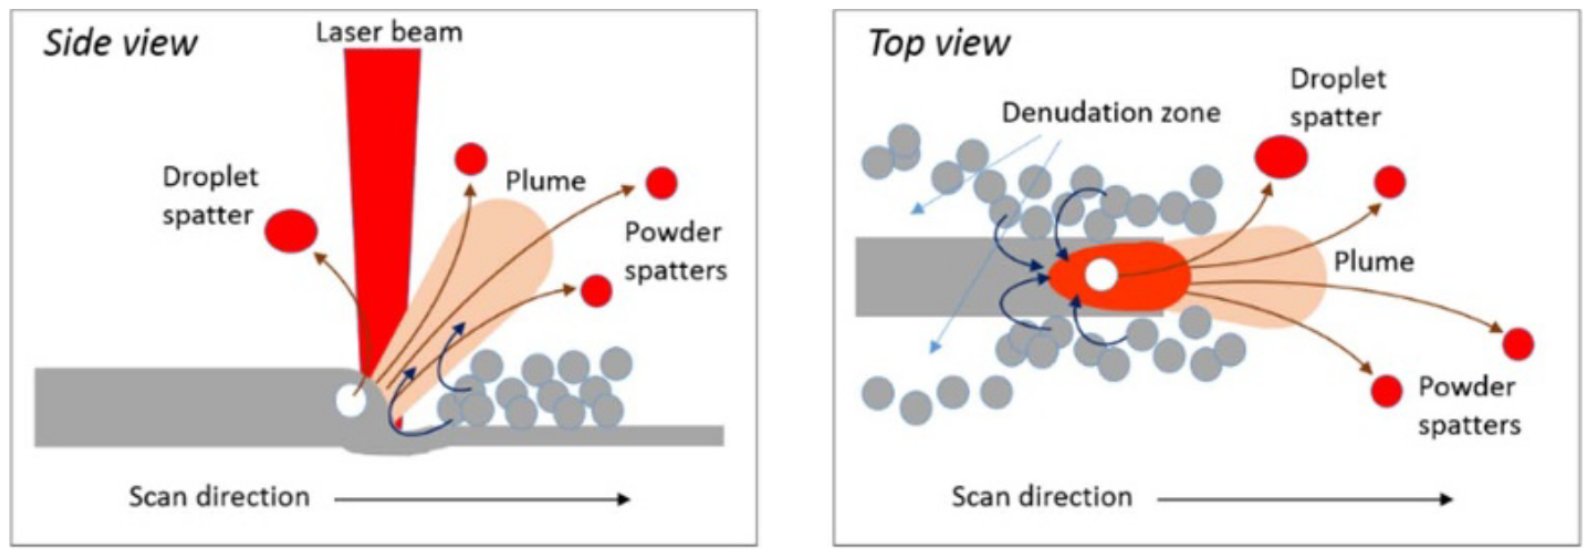
\includegraphics[width = 0.6\textwidth]{Images/plume.png}
    \caption[Spatters and plume in SLS]{Schematic representation of spatters and plume emission in SLS \cite{grasso_-situ_2021}}
    \label{fig:plume}
\end{figure}

\begin{figure}
    \centering
    \subfloat[\label{fig:colosimoplume}]{
        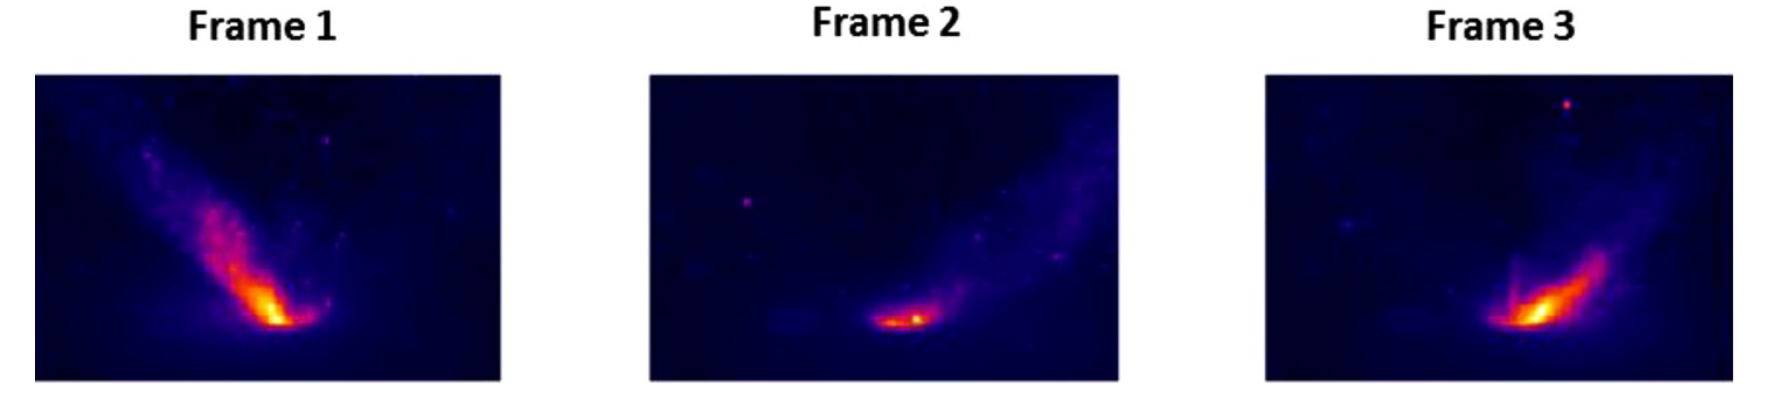
\includegraphics[scale=0.4]{Images/plumecolosimo.png}
    }
    \qquad
    \subfloat[\label{fig:barretspatter}]{
        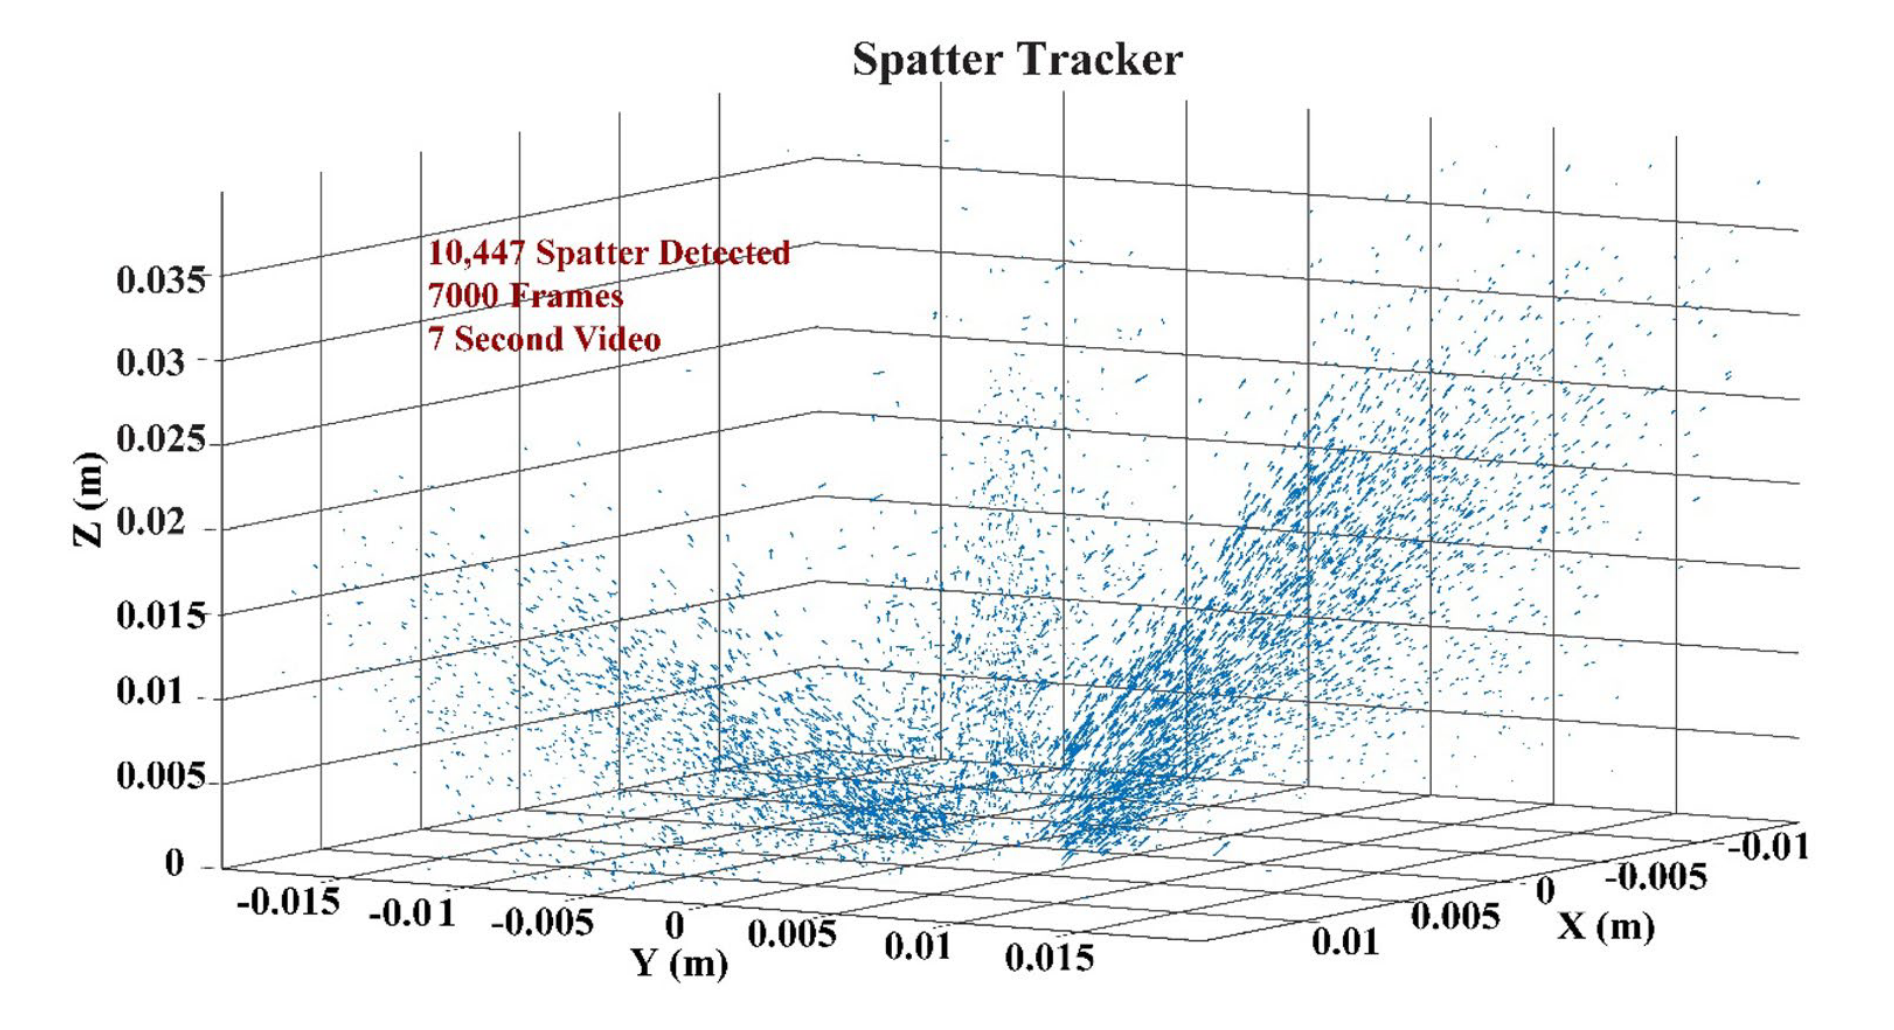
\includegraphics[scale=0.3]{Images/splatter.png}
    }
    \caption[Methods for plume and spatter detection.]{Methods for plume and spatter detection: plume emissions captured with long wave IR video imaging (a) \cite{grasso_statistical_2019} and 3D spatter localisation via high-speed stereo vision (b) \cite{barrett_statistical_2019}.}
\end{figure}
\paragraph{Measurement of air-borne acoustic emission.} In L-PBF processes, there is a research streams that involves airborne acoustic emission sensors. The measurement system consists of capturing air density variations during the laser scanning by placing the sensor in the roximity of melted area. To measure acoustic vibration, we can use Bragg grating optoacoustic sensor installed into the build chamber at about \SI{200}{\milli\metre} from the process zone, with a sampling frequency of \SI{1}{\mega\hertz}. In \citeauthor{wasmer_situ_2019} (2019), the sensor was placed so that the longitudinal axis of the fibre was perpendicular to the acoustic wave to increase its sensitivity. We can also use more common sensors like in \citeauthor{ye_defect_2018} (2018). In the study, authors installed a microphone into the build chamber at an angle of \SI{30}{\degree} above the build area, with a frequency response in the range \SIrange[range-phrase=--]{0}{100}{\kilo\hertz}. The resulting measurements and their information content in the temporal and/or frequency domain can be viewed as signatures of the laser-material interaction.
\begin{figure}
    \centering
    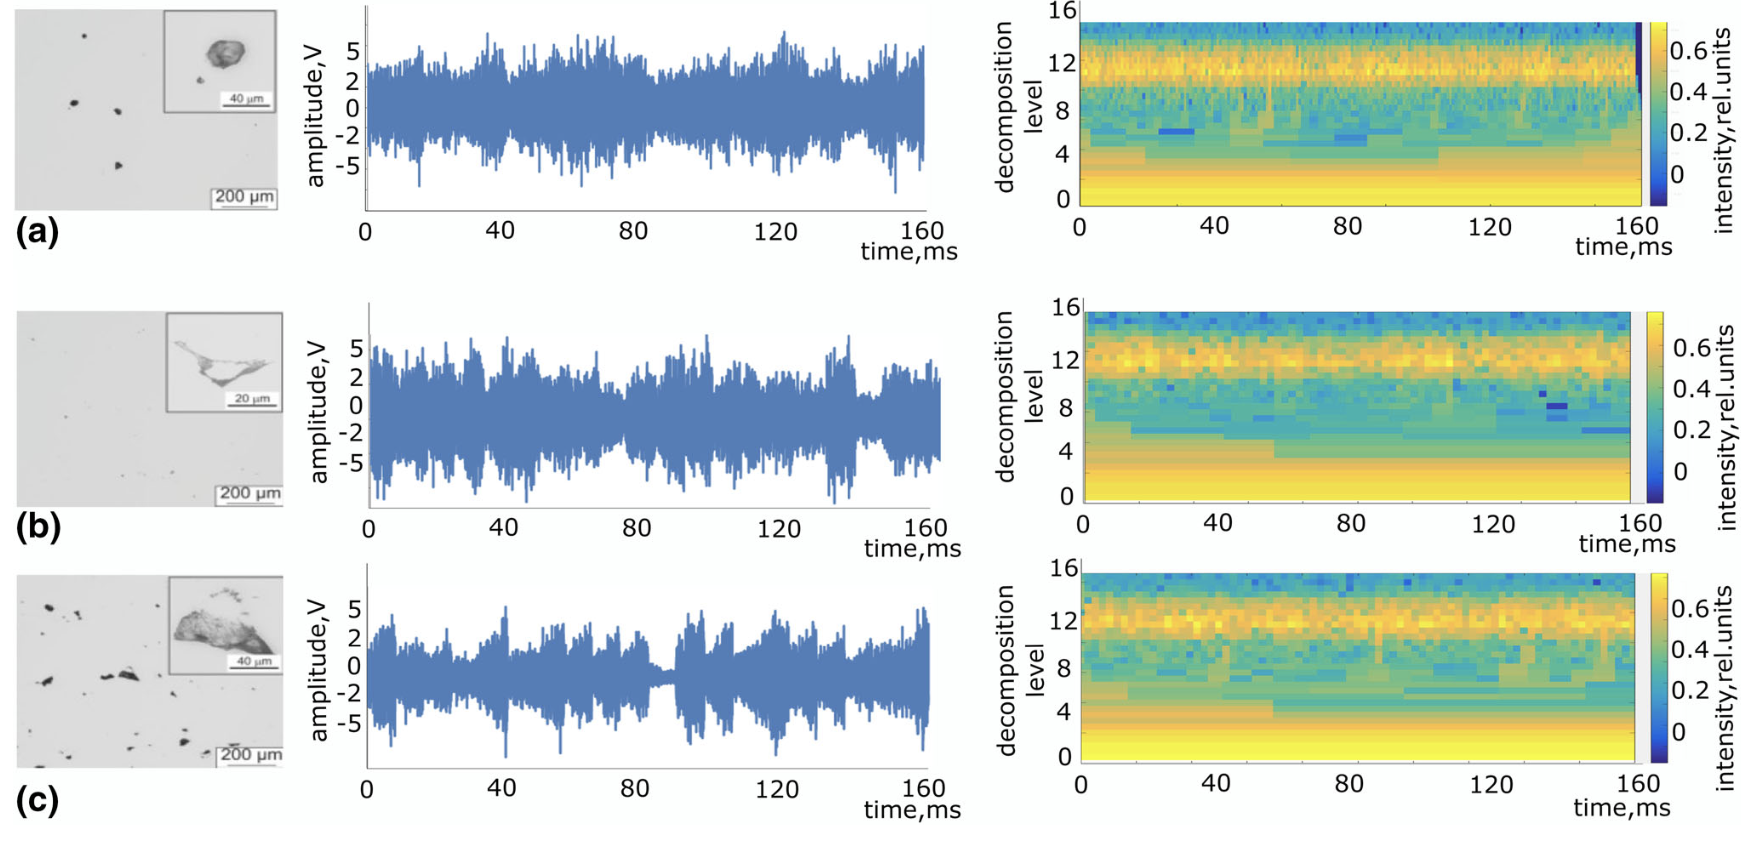
\includegraphics[width = 0.8\textwidth]{Images/acustic.png}
    \caption[Example of AE of different porosities specimens.] {From left to right, typical light microscope cross-sectional images with different porosities, their corresponding acoustic emission signals with a \SI{160}{\milli\second} time span, and their corresponding wavelet spectrogram of the regions produced with different scanned velocity \SI{300}{\milli\metre / \second} (a), \SI{500}{\milli\metre / \second} (b) and \SI{800}{\milli\metre /\second} (c) \cite{wasmer_situ_2019}}
    \label{fig:acustic}
\end{figure}


\textcolor{red}{Manca livello 3.}
All the layers discussed so far have one common element: all of them are used for monitoring of the last printed layer, either before, during or after the melting phase. For \emph{level ~4}, the subject of the monitoring process is under the last layer. Indeed, as the next layer is being printed, the material characteristics underneath are modified as well, due to partial remelting of top layers and heat exchanges within the build volume. Since it's evident that we cannot use optical devices to monitor what we cannot see, level 4 monitoring relies on other sensors. We ca use high-speed high-energy x-ray imaging systems the gain information about the energy penetration depth and pore formation, or we can use x-ray diffraction measurement to detect any strain and stress formation. Fig. \ref{fig:xray4} shows the result of an x-ray video imaging in L-PBF. Moreover, in last years a new research streams about in-situ x-ray micro-tomography was born. In \citeauthor{lhuissier_situ_2020}, during the in-situ microtomography scan, 1500 projections were acquired resulting in a scan time of \SI{45}{s}, gathering a spatial resolution of \SI{3.64}{\micro\metre / pixel}. A field of research with a direct application potentials in industry regards the in-situ measurements of acoustic emissions (AEs) and specifically of structure-borne AEs. These AEs  are suitable to detect sudden releases of elastic energy that propagate within the material, which means that allow us to detect crack formations, detachments of overhang areas from supports or delamination phenomena. We can also use multiple sensors placed at different location in order to triangulate the position of the epicenter of the energy release. A pioneer in the use of AEs in PBF processes is Rieder. In \citeauthor{rieder_-_2016} (2016) he proposed an ultrasonic monitoring device in L-PBF mounted on the underside of the baseplate focusing on the bottom plate interface echo and the backwall echo patterns as proxies of discontinuities in the specimen.
\begin{figure}
    \centering
    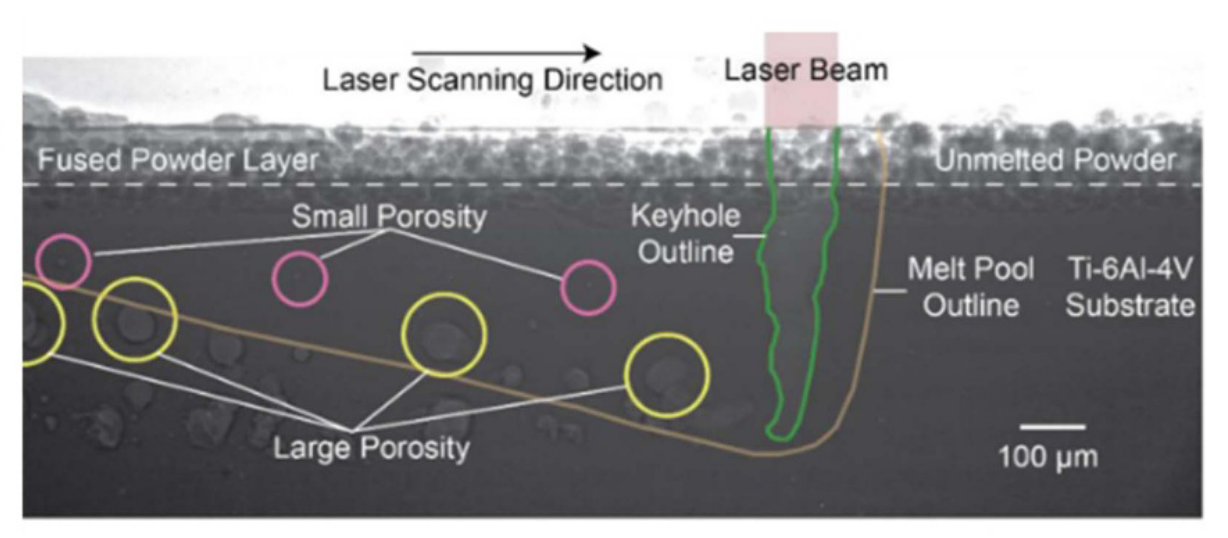
\includegraphics[width=0.65\textwidth]{Images/xray4.png}
    \caption[X-ray video frame.]{Example of an in-situ x-ray video frame with relative defects identified \cite{paulson_correlations_2020}.}
    \label{fig:xray4}
\end{figure}
% <<< End of Sensors for anomalies detection